\documentclass[11pt,a4paper]{article}

% ------------------------------------------------------------------ details --
% >>> Edit these before submitting <<<
\newcommand{\studentname}{Rajinthan R.}
\newcommand{\indexno}{220502M}
\newcommand{\codeurl}{https://github.com/rajinthanr/en3330-lagrangian-duality}
\newcommand{\submitdate}{19 October 2026}

% ----------------------------------------------------------------- packages --
\usepackage{amsmath}
\usepackage[T1]{fontenc}
\usepackage{newtxtext,newtxmath}
\usepackage[margin=2.5cm,headheight=14pt]{geometry}
\usepackage{microtype}
\usepackage{graphicx}
\usepackage{float}
\usepackage{booktabs}
\usepackage{caption}
\usepackage{subcaption}
\usepackage{enumitem}
\usepackage{xcolor}
\usepackage{fancyhdr}
\usepackage{titlesec}
\usepackage{listings}
\usepackage[most]{tcolorbox}
\usepackage[hidelinks]{hyperref}
\usepackage[capitalise,noabbrev]{cleveref}

\graphicspath{{../figures/}}
\linespread{1.1}
\setlength{\parskip}{0.45em}
\setlength{\parindent}{0pt}
\captionsetup{font=small,labelfont=bf,margin=0.5cm}
\setlist{itemsep=0.2em,topsep=0.3em}

\definecolor{accent}{HTML}{1F4E8C}
\definecolor{codebg}{HTML}{F6F6F4}
\definecolor{codegray}{HTML}{6B6A66}
\definecolor{codegreen}{HTML}{2E7D32}

\titleformat{\section}{\large\bfseries\color{accent}}{\thesection}{0.8em}{}
\titleformat{\subsection}{\normalsize\bfseries}{\thesubsection}{0.6em}{}
\titlespacing*{\section}{0pt}{1.2em}{0.5em}
\titlespacing*{\subsection}{0pt}{0.9em}{0.3em}

\pagestyle{fancy}
\fancyhf{}
\lhead{\small EN3330 -- Assignment 03}
\rhead{\small \studentname\ (\indexno)}
\cfoot{\small \thepage}
\renewcommand{\headrulewidth}{0.4pt}

\newtcolorbox{resultbox}{colback=accent!5,colframe=accent!60,boxrule=0.5pt,
  arc=2pt,left=6pt,right=6pt,top=4pt,bottom=4pt}

\lstset{
  language=Python, basicstyle=\ttfamily\scriptsize, backgroundcolor=\color{codebg},
  keywordstyle=\color{accent}\bfseries, commentstyle=\color{codegray}\itshape,
  stringstyle=\color{codegreen}, numbers=left, numberstyle=\tiny\color{codegray},
  breaklines=true, frame=single, rulecolor=\color{codegray!40}, columns=fullflexible,
  showstringspaces=false, upquote=true}

\newcommand{\Lag}{\mathcal{L}}
\DeclareMathOperator*{\argmin}{arg\,min}
\DeclareMathOperator*{\argmax}{arg\,max}

% ================================================================= document ==
\begin{document}

% ---------------------------------------------------------------- title page --
\begin{titlepage}
  \thispagestyle{empty}
  \centering
  \vspace*{0.5cm}
  
\includegraphics[width=0.22\textwidth]{uom_logo.png}\par
  \vspace{0.6cm}
  {\large University of Moratuwa\par}
  {\normalsize Department of Electronic and Telecommunication Engineering\par}
  \vspace{1.6cm}
  {\large\bfseries EN3330\par}
  \vspace{0.6cm}
  {\color{accent}\rule{0.7\textwidth}{0.8pt}\par}
  \vspace{0.4cm}
  {\Huge\bfseries Assignment 03\par}
  \vspace{0.3cm}
  {\Large Lagrangian Duality, Saddle Points\\[0.15em] and Weak Duality\par}
  \vspace{0.4cm}
  {\color{accent}\rule{0.7\textwidth}{0.8pt}\par}
  \vspace{2cm}
  \begin{tabular}{@{}ll@{}}
    \textbf{Name}         & \studentname \\[0.3em]
    \textbf{Index number} & \indexno \\[0.3em]
    \textbf{Date}         & \submitdate \\
  \end{tabular}
  \vfill
  {\small \textbf{Source code:} \url{\codeurl}\par}
  \vspace{1cm}
\end{titlepage}

% ------------------------------------------------------------------ overview --
\section*{Overview}

All three questions are based on the same problem,
\begin{equation}
  \min_x\; f(x)=x^2 \quad\text{subject to}\quad h(x)=1-x\le 0,
  \qquad
  \Lag(\mu,x)=x^2+\mu(1-x),\;\; \mu\ge 0 .
  \label{eq:problem}
\end{equation}
The answer to the primal problem is clear. Since $x^2$ is increasing on
$[1,\infty)$, the smallest value is at $x^*=1$, and $p^*=f(x^*)=1$. In this
report, the same problem is studied using the Lagrangian.

All the figures were drawn using one Python script (NumPy and Matplotlib). The
same script also checks every analytical result numerically, using grid
search. The results of these checks are given in the relevant sections, and
the full output is given in \cref{app:log}.

\begin{resultbox}
\textbf{Source code:} \url{\codeurl}\\
File \texttt{src/duality\_simulation.py}. It can be run using
\texttt{python3 src/duality\_simulation.py}. The full code is given in \cref{app:code}.
\end{resultbox}

% =================================================================== Q1 ====
\section{The Lagrangian, the dual function and the primal function}

\subsection{(a) $\Lag(\mu,x)$ as a function of $x$}

When $\mu$ is fixed, $\Lag(\mu,\cdot)$ is a convex parabola in $x$. Its
minimum point is found by setting the derivative to zero:
\begin{equation}
  \frac{\partial \Lag}{\partial x}=2x-\mu=0
  \;\;\Longrightarrow\;\;
  x(\mu)=\argmin_x \Lag(\mu,x)=\frac{\mu}{2},
  \qquad
  \Lag\bigl(\mu,x(\mu)\bigr)=\mu-\frac{\mu^2}{4}.
  \label{eq:xmu}
\end{equation}

\begin{figure}[!htbp]
  \centering
  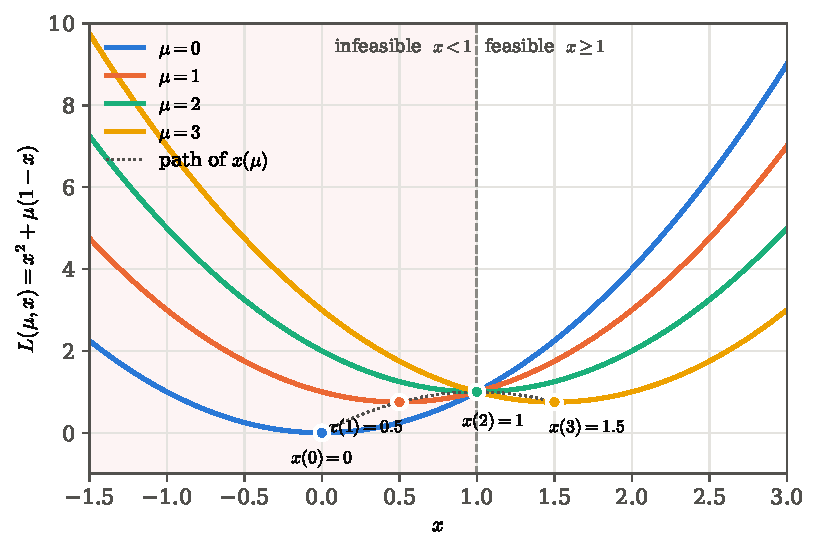
\includegraphics[width=0.82\textwidth]{q1a_lagrangian_vs_x.pdf}
  \caption{$\Lag(\mu,x)=x^2+\mu(1-x)$ for $\mu=0,1,2,3$. The dots show the
  minimum points $x(\mu)=\mu/2$. The shaded area is not feasible ($x<1$). The
  dotted curve shows how the minimum point moves when $\mu$ changes.}
  \label{fig:q1a}
\end{figure}

\begin{table}[!htbp]
  \centering
  \caption{Minimum points of $\Lag(\mu,\cdot)$. The values from the formula
  are the same as the values from a grid search over $x\in[-10,10]$ with step
  $5\times10^{-5}$.}
  \label{tab:q1a}
  \begin{tabular}{@{}cccc@{}}
    \toprule
    $\mu$ & $x(\mu)=\mu/2$ & $\min_x\Lag(\mu,x)$ & Feasible? \\
    \midrule
    0 & 0.0 & 0.00 & no \\
    1 & 0.5 & 0.75 & no \\
    2 & 1.0 & 1.00 & yes (on the boundary) \\
    3 & 1.5 & 0.75 & yes (inside) \\
    \bottomrule
  \end{tabular}
\end{table}

\textbf{How the minimum point moves.} When $\mu$ increases, the minimum point
$x(\mu)=\mu/2$ moves to the right. It moves by $1/2$ for every unit increase
in $\mu$ (\cref{fig:q1a}). The term $\mu(1-x)$ adds a cost to the points with
$x<1$ and reduces the cost of the points with $x>1$. Because of this, the
lowest point of the parabola moves towards the feasible region.
\begin{itemize}
  \item When $\mu<2$, the minimum point is still not feasible ($x(\mu)<1$).
        The value of $\mu$ is not large enough.
  \item When $\mu=2$, the minimum point is exactly on the boundary,
        $x(2)=1=x^*$.
  \item When $\mu>2$, the minimum point goes inside the feasible region. It
        is feasible, but it is not the optimal point. The value of $\mu$ is
        too large.
\end{itemize}
It can also be seen that all the curves go through the point $(1,1)$. The
reason is that $h(1)=0$, so $\Lag(\mu,1)=1$ for every $\mu$. On the boundary,
the value of $\mu$ does not change the Lagrangian.

\subsection{(b) The dual function}

By substituting $x(\mu)$ from \eqref{eq:xmu} into the Lagrangian,
\begin{equation}
  d(\mu)=\min_x \Lag(\mu,x)=\Bigl(\frac{\mu}{2}\Bigr)^2+\mu\Bigl(1-\frac{\mu}{2}\Bigr)
        =\mu-\frac{\mu^2}{4},\qquad \mu\ge 0 .
  \label{eq:dual}
\end{equation}
Since $d''(\mu)=-\tfrac12<0$, the dual function is a concave parabola. To find
its maximum,
\begin{equation}
  d'(\mu)=1-\frac{\mu}{2}=0 \;\Longrightarrow\;
  \boxed{\mu^*=2,\qquad d^*=d(2)=1.}
\end{equation}
This value satisfies $\mu^*\ge 0$, so the condition $\mu\ge0$ does not affect
the answer. A grid search over $\mu\in[0,10]$ gives the same values
(\cref{app:log}).

\begin{figure}[!htbp]
  \centering
  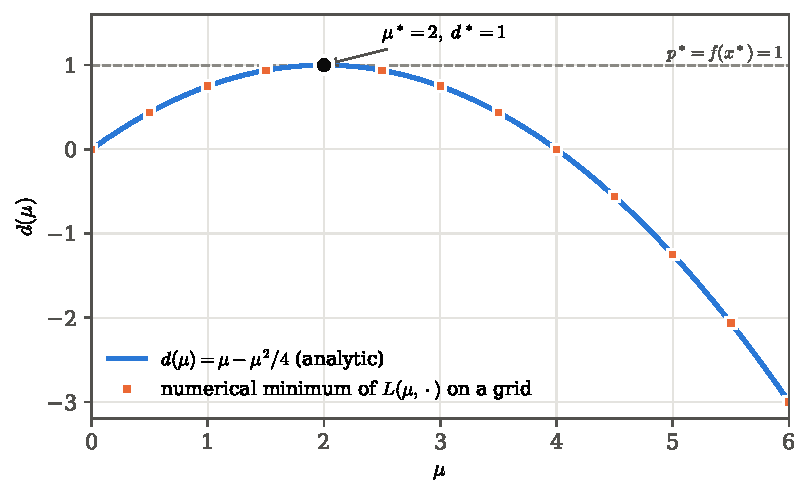
\includegraphics[width=0.8\textwidth]{q1b_dual_function.pdf}
  \caption{Dual function $d(\mu)=\mu-\mu^2/4$ (line) and the values from the
  numerical minimisation of $\Lag(\mu,\cdot)$ (squares). The maximum value
  $d^*=1$ at $\mu^*=2$ is equal to the primal optimal value $p^*=1$ (dashed
  line).}
  \label{fig:q1b}
\end{figure}

\textbf{Discussion.} For every $\mu$, $d(\mu)\le 1$, and the maximum value is
exactly $p^*=1$. Therefore the \emph{duality gap is zero}. This is the
expected result. The problem is convex ($f$ is convex and $h$ is linear), and
there is a point which satisfies the constraint strictly (for example $x=2$
gives $h(2)<0$). So Slater's condition is satisfied, and strong duality
holds. It can also be seen that $\mu^*=2$ is the same value of $\mu$ for which
the minimum point in part (a) is at $x^*=1$. That is, $x(\mu^*)=x^*$.

The value of $\mu^*$ also has a practical meaning. Suppose the constraint is
changed to $x\ge b$ with $b\ge 0$. Then the optimal value is $p^*(b)=b^2$, and
$\mathrm{d}p^*/\mathrm{d}b=2b=2=\mu^*$ at $b=1$. This means that if the
constraint is made tighter by a small amount $\delta$, the optimal cost
increases by about $2\delta$. For this reason, $\mu^*$ is called the
``shadow price'' of the constraint.

\subsection{(c) The primal function}

When $x$ is fixed, $\Lag(\mu,x)=x^2+\mu(1-x)$ is a straight line in $\mu$
with slope $1-x=h(x)$. Therefore, the maximum over $\mu\ge 0$ is
\begin{equation}
  g(x)=\max_{\mu\ge 0}\Lag(\mu,x)=x^2+\sup_{\mu\ge0}\mu(1-x)
  =\begin{cases}
     x^2, & x\ge 1 \quad (\text{slope}\le 0,\ \text{best } \mu=0),\\[0.2em]
     +\infty, & x<1 \quad (\text{slope}>0,\ \mu\to\infty).
   \end{cases}
  \label{eq:primal}
\end{equation}

To show this using a graph, \cref{fig:q1c} plots
$g_M(x)=\max_{0\le\mu\le M}\Lag(\mu,x)$ for larger and larger values of $M$.
\begin{itemize}
  \item In the feasible region ($x\ge1$), all the curves are the same as
        $x^2$ for any value of $M$.
  \item In the infeasible region ($x<1$), $g_M(x)=x^2+M(1-x)$ becomes larger
        and larger when $M$ increases. It goes to $+\infty$ when
        $M\to\infty$.
\end{itemize}
The values in \cref{tab:q1c} show the same result. At $x=0$ the value is
equal to $M$. Even at $x=0.99$, the value keeps increasing with $M$.

\begin{figure}[!htbp]
  \centering
  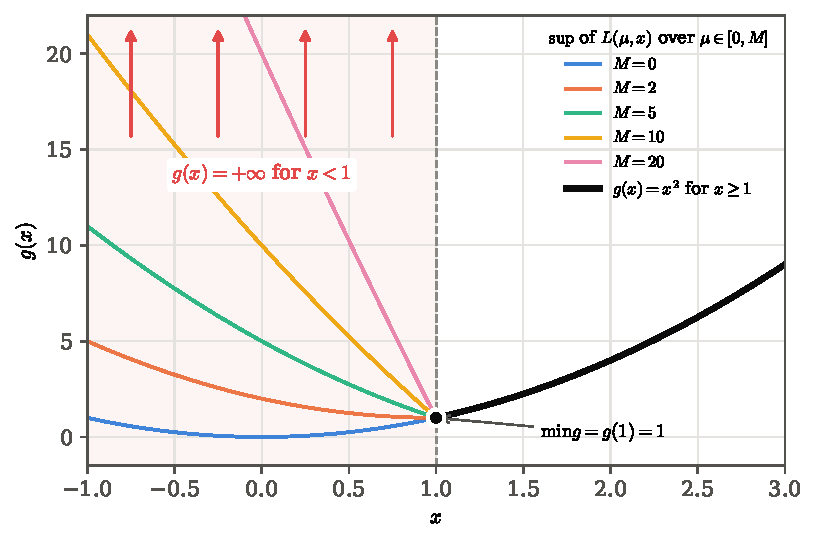
\includegraphics[width=0.82\textwidth]{q1c_primal_function.pdf}
  \caption{Primal function. The coloured curves are
  $\max_{0\le\mu\le M}\Lag(\mu,x)$ for different values of $M$. They are equal
  to $x^2$ when $x\ge 1$ and go to infinity when $x<1$. Therefore
  $g(x)=x^2+I_{\{x\ge1\}}(x)$. Its minimum is at $x=1$, where $g(1)=1$.}
  \label{fig:q1c}
\end{figure}

\begin{table}[!htbp]
  \centering
  \caption{Values of $\max_{0\le\mu\le M}\Lag(\mu,x)$ from the simulation.}
  \label{tab:q1c}
  \begin{tabular}{@{}crrrrr@{}}
    \toprule
    $x$ & $M=1$ & $M=10$ & $M=100$ & $M=1000$ & $x^2$ \\
    \midrule
    $-1.00$ & 3.00 & 21.00 & 201.00 & 2001.00 & 1.00 \\
    $0.00$  & 1.00 & 10.00 & 100.00 & 1000.00 & 0.00 \\
    $0.99$  & 0.99 & 1.08  & 1.98   & 10.98   & 0.98 \\
    $1.00$  & 1.00 & 1.00  & 1.00   & 1.00    & 1.00 \\
    $2.00$  & 4.00 & 4.00  & 4.00   & 4.00    & 4.00 \\
    \bottomrule
  \end{tabular}
\end{table}

\textbf{Why $\min_x g(x)$ is the same as problem (1).} From
\eqref{eq:primal}, $g = f + I_{\mathcal F}$. Here $I_{\mathcal F}$ is $0$ on
the feasible set $\mathcal F=\{x\ge 1\}$ and $+\infty$ outside it. Every
infeasible point has an infinite value, so it cannot be the minimum of $g$.
Inside $\mathcal F$, $g$ is the same as the original objective. Therefore,
\[
  \min_x g(x)=\min_{x\ge 1} x^2 = p^* = 1, \qquad \argmin_x g = x^* = 1 .
\]
Both problems have the same minimum point and the same minimum value. In other
words, the constrained problem can be written as a problem without
constraints, $p^*=\min_x\max_{\mu\ge0}\Lag(\mu,x)$. The dual problem in part
(b) is the same expression with the order changed,
$d^*=\max_{\mu\ge0}\min_x\Lag(\mu,x)$. For this problem, both orders give
the same value, $d^*=p^*=1$.

% =================================================================== Q2 ====
\section{Saddle point of the Lagrangian}

In this question, $x^*=1$ and $\mu^*=2$ from Question 1 are used.

\subsection{(a) $(x^*,\mu^*)$ is a saddle point}

\begin{enumerate}[label=(\roman*),leftmargin=2.2em]
  \item $\Lag(\mu^*,x^*)=1^2+2(1-1)=\boxed{1}.$

  \item $\Lag(\mu,x^*)=1^2+\mu(1-1)=1$ for every $\mu\ge 0$. This does not
        depend on $\mu$, because the constraint is active at $x^*$
        ($h(x^*)=0$). So the term with $\mu$ becomes zero. Therefore,
        \[
          \Lag(\mu,x^*)=1\le 1=\Lag(\mu^*,x^*)\qquad\forall\,\mu\ge0,
        \]
        and the left inequality is satisfied (with equality).

  \item $\Lag(\mu^*,x)=x^2+2(1-x)=x^2-2x+2=(x-1)^2+1.$ Since
        $(x-1)^2\ge 0$,
        \[
          \Lag(\mu^*,x)=(x-1)^2+1\ge 1=\Lag(\mu^*,x^*)\qquad\forall\,x.
        \]
        Equality is only at $x=x^*=1$. Therefore the right inequality is also
        satisfied.

  \item The two graphs are shown in \cref{fig:q2a}. Both graphs go through
        the common value $\Lag(\mu^*,x^*)=1$. In the $\mu$ direction, the
        Lagrangian is constant, so $\mu^*$ is a maximum point (but not the only
        one). In the $x$ direction, it is a parabola with its minimum at
        $x^*$.
\end{enumerate}

\begin{figure}[!htbp]
  \centering
  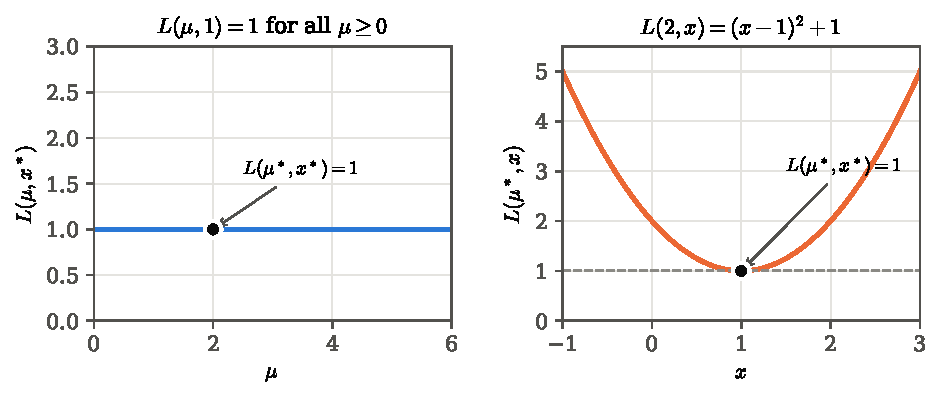
\includegraphics[width=0.95\textwidth]{q2a_saddle_slices.pdf}
  \caption{$\Lag$ through the saddle point. Left: $\Lag(\mu,x^*)$ is always
  equal to 1. Right: $\Lag(\mu^*,x)=(x-1)^2+1$ has its minimum value of 1 at
  $x^*=1$. The black dot shows the common value $\Lag(\mu^*,x^*)=1$.}
  \label{fig:q2a}
\end{figure}

\Cref{fig:q2a-contour} shows the whole function as a contour plot. The
contour $\Lag=1$ is made of two lines, $x=1$ and $x=\mu-1$. These two lines
cross at $(\mu^*,x^*)=(2,1)$, which is the usual shape near a saddle point.
Both inequalities were also checked numerically for $\mu\in[0,50]$ and
$x\in[-20,20]$. The results were $\max_\mu\Lag(\mu,x^*)=1$ and
$\min_x\Lag(\mu^*,x)=1$. The largest difference between $\Lag(2,x)$ and
$(x-1)^2+1$ was about $10^{-13}$, which is only a rounding error.

\begin{figure}[!htbp]
  \centering
  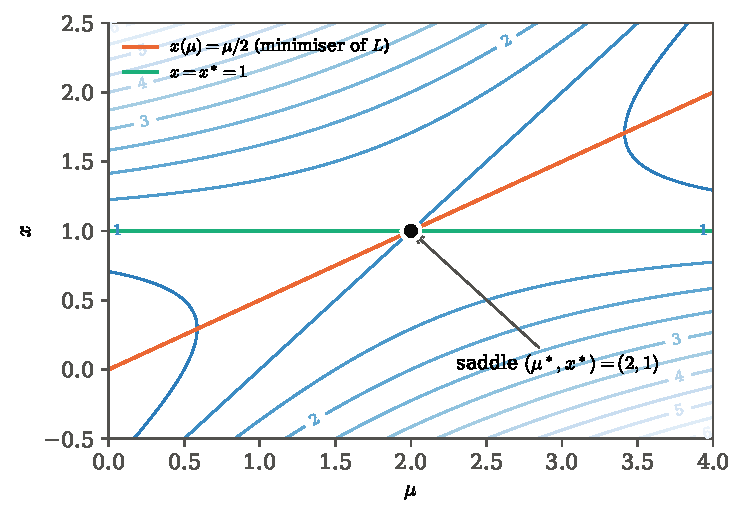
\includegraphics[width=0.66\textwidth]{q2a_saddle_contour.pdf}
  \caption{Contour plot of $\Lag(\mu,x)$. The line of minimum points
  $x(\mu)=\mu/2$ meets the line $x=x^*$ exactly at the saddle point $(2,1)$.}
  \label{fig:q2a-contour}
\end{figure}

\subsection{(b) Why the saddle point is optimal}

For any feasible $x$ (that is, $h(x)\le 0$),
\[
  f(x^*) \overset{(1)}{=} \Lag(\mu^*,x^*) \overset{(2)}{\le} \Lag(\mu^*,x)
  \overset{(3)}{=} f(x)+\mu^* h(x) \overset{(4)}{\le} f(x).
\]
\begin{enumerate}[label=(\arabic*),leftmargin=2.2em]
  \item $\Lag(\mu^*,x^*)=f(x^*)+\mu^*h(x^*)$, and $\mu^*h(x^*)=0$ because
        $h(x^*)=0$ (complementary slackness).
  \item This is the right inequality of the saddle point. $x^*$ gives the
        minimum of $\Lag(\mu^*,\cdot)$ over \emph{all} $x$, so it is also the
        minimum over the feasible $x$.
  \item This is the definition of the Lagrangian.
  \item $\mu^*\ge 0$, and $h(x)\le 0$ for a feasible $x$. So $\mu^*h(x)\le 0$.
\end{enumerate}
Therefore $f(x^*)\le f(x)$ for every feasible $x$, and $x^*$ is the global
minimum. Convexity is not used in this proof. So \emph{any} saddle point of the
Lagrangian gives an optimal solution of the primal problem.

\textbf{What the left inequality says about $h(x^*)$.} The left inequality is
\[
  f(x^*)+\mu\,h(x^*) \le \Lag(\mu^*,x^*) < \infty \qquad \forall\,\mu\ge 0 .
\]
If $h(x^*)>0$, the left side goes to $+\infty$ when $\mu\to\infty$. But the
right side is a finite number, so this is not possible. Therefore
$h(x^*)\le 0$. This means that \emph{the left inequality makes sure that $x^*$
is feasible.} This is the same idea as the primal function $g$ in Q1(c).

\textbf{What it says about $\mu^*h(x^*)$.} If $\mu=0$ is used in the left
inequality, $f(x^*)\le f(x^*)+\mu^*h(x^*)$, so $\mu^*h(x^*)\ge 0$. Also,
$\mu^*\ge0$ and $h(x^*)\le0$, so $\mu^*h(x^*)\le 0$. From these two results,
$\mu^*h(x^*)=0$. So the left inequality also gives the complementary
slackness condition. It also means that $\mu^*$ gives the maximum of
$\Lag(\cdot,x^*)$ over $\mu\ge 0$.

\subsection{(c) Complementary slackness and an inactive constraint}

\textbf{Original problem.} $\mu^*h(x^*)=2\,(1-1)=0$, so the complementary
slackness condition is satisfied. In this case the constraint is active
($h(x^*)=0$) and the multiplier is positive. The constraint actually stops the
solution from going to the unconstrained minimum $x=0$.

\textbf{New constraint $x\ge -1$}, that is, $h(x)=-1-x\le 0$.
\begin{itemize}
  \item \emph{Is $x=0$ feasible?} Yes. $0\ge -1$, or $h(0)=-1\le 0$. So the
        unconstrained minimum of $x^2$ is also the constrained minimum:
        $x^*=0$ and $p^*=0$.
  \item \emph{Is the constraint active?} No. $h(0)=-1<0$, so the constraint
        is satisfied with a strict inequality at the optimum.
  \item \emph{Expected value of $\mu^*$: $\mu^*=0$.} From complementary
        slackness, $\mu^*h(x^*)=\mu^*\cdot(-1)=0$, so $\mu^*=0$. The
        stationarity condition gives the same answer:
        $\partial_x\Lag=2x^*-\mu^*=0$ at $x^*=0$, so $\mu^*=0$. Also, if the
        bound $-1$ is changed by a small amount, the optimal cost does not
        change ($p^*$ is still $0$). So the shadow price is zero. Since an
        inactive constraint does not affect the solution, its multiplier is
        zero.
\end{itemize}

\textbf{What the left inequality says about $\mu^*$.} With $x^*=0$,
$\Lag(\mu,x^*)=0+\mu(-1-0)=-\mu$. So the left inequality becomes
$-\mu\le-\mu^*$ for all $\mu\ge0$, that is, $\mu^*\le\mu$ for every
$\mu\ge 0$. When $\mu=0$, this gives $\mu^*\le 0$. Since $\mu^*\ge 0$ as well,
$\mu^*=0$. So in this case, the left inequality gives only one possible value
for the multiplier. In the active case, the left inequality was satisfied with
equality for every $\mu$.

The dual function gives the same result. Again $x(\mu)=\mu/2$, and
$d(\mu)=\mu^2/4+\mu(-1-\mu/2)=-\mu-\mu^2/4$. This function decreases for all
$\mu\ge0$, so $\mu^*=0$ and $d^*=0=p^*$ (\cref{fig:q2c}). The numerical values
(squares) are the same as the formula.

\begin{figure}[!htbp]
  \centering
  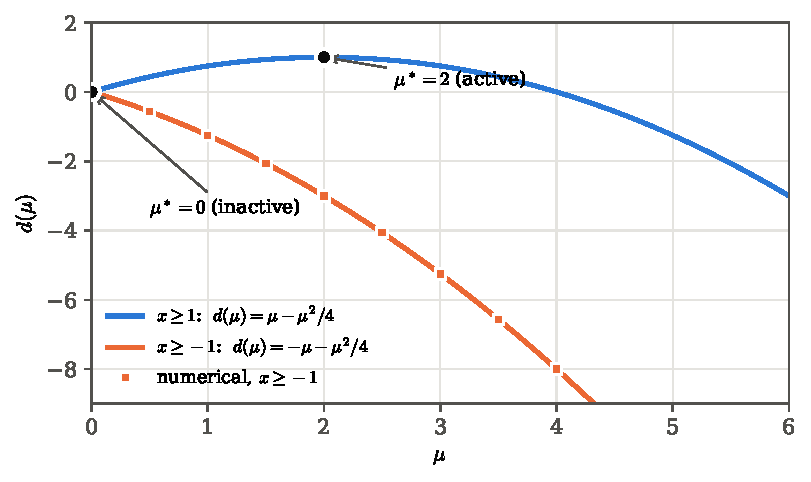
\includegraphics[width=0.8\textwidth]{q2c_modified_dual.pdf}
  \caption{Dual functions for the active constraint $x\ge1$ (maximum at
  $\mu^*=2$) and for the inactive constraint $x\ge-1$ (maximum at
  $\mu^*=0$).}
  \label{fig:q2c}
\end{figure}

% =================================================================== Q3 ====
\section{Weak duality}

\subsection{(a) $d(\mu)\le p^*$}

Let $\mu\ge0$, and let $x$ be any feasible point, so $h(x)\le 0$. Then
\[
  d(\mu)\overset{(1)}{\le}\Lag(\mu,x)=f(x)+\mu h(x)\overset{(2)}{\le}f(x).
\]
\begin{enumerate}[label=(\arabic*),leftmargin=2.2em]
  \item $d(\mu)$ is the minimum of $\Lag(\mu,\cdot)$ over \emph{all} $x$. So
        it cannot be larger than the value of $\Lag(\mu,\cdot)$ at any one
        point $x$.
  \item $\mu\ge0$ and $h(x)\le0$, so $\mu h(x)\le0$.
\end{enumerate}
The result $d(\mu)\le f(x)$ is true for \emph{every} feasible $x$. So it is
also true for the smallest value of $f(x)$. Taking the minimum over all
feasible $x$,
\[
  d(\mu)\le \min_{h(x)\le0}f(x)=p^*\qquad\forall\,\mu\ge 0 .
\]
Convexity is not used here, so weak duality is true for every problem.

\textbf{Numerical check for Question 1}, using $d(\mu)=\mu-\mu^2/4$ and $p^*=1$:

\begin{table}[!htbp]
  \centering
  \caption{Weak duality check. All the dual values are less than or equal to
  $p^*=1$, and the gap becomes zero at $\mu^*=2$.}
  \label{tab:weak}
  \begin{tabular}{@{}ccccc@{}}
    \toprule
    $\mu$ & $d(\mu)=\mu-\mu^2/4$ & $p^*$ & gap $p^*-d(\mu)$ & $d(\mu)\le p^*$? \\
    \midrule
    0 & 0.00 & 1 & 1.00 & \checkmark \\
    1 & 0.75 & 1 & 0.25 & \checkmark \\
    2 & 1.00 & 1 & 0.00 & \checkmark \;(equal) \\
    3 & 0.75 & 1 & 0.25 & \checkmark \\
    \bottomrule
  \end{tabular}
\end{table}

In general, $p^*-d(\mu)=1-\mu+\mu^2/4=(1-\mu/2)^2\ge0$. So the result is true
for every $\mu$, not only for these four values. The simulation also shows that
$\max_{\mu\in[0,100]}d(\mu)=1\le p^*$. This means that any value of $d(\mu)$
gives a lower bound for the optimal cost, even without solving the primal
problem.

\subsection{(b) Lower envelope and concavity of $d$}

When $x$ is fixed, $\Lag(\mu,x)=x^2+\mu(1-x)$ is a straight line in $\mu$.
Its intercept is $x^2$ and its slope is $1-x$:
\[
  x=0:\ \Lag=\mu,\qquad x=1:\ \Lag=1,\qquad x=2:\ \Lag=4-\mu .
\]
The lower envelope of these three lines is
\[
  \min\{\mu,\,1,\,4-\mu\}=
  \begin{cases}\mu, & 0\le\mu\le1,\\ 1, & 1\le\mu\le3,\\ 4-\mu, & \mu\ge3.\end{cases}
\]

\begin{figure}[!htbp]
  \centering
  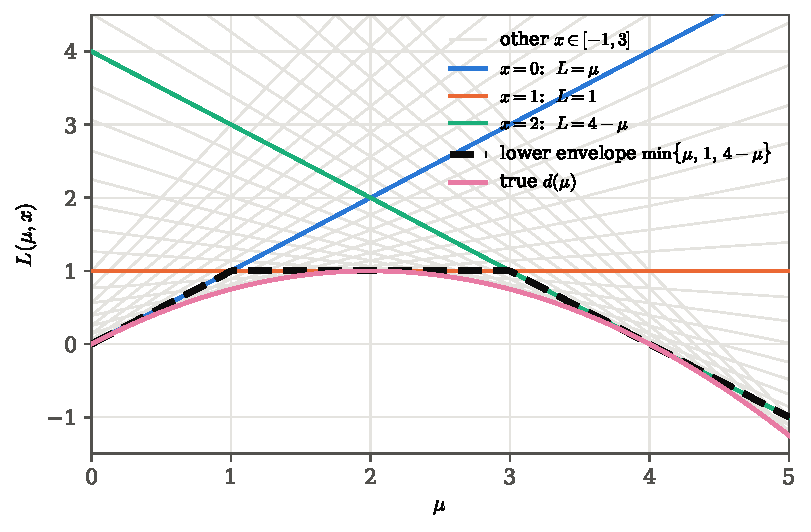
\includegraphics[width=0.82\textwidth]{q3b_lower_envelope.pdf}
  \caption{$\Lag(\mu,x)$ against $\mu$ for $x=0,1,2$ (coloured lines) and for
  33 other values of $x\in[-1,3]$ (light grey). The dashed line is the lower
  envelope of the three coloured lines. It is made of straight pieces, it is
  concave, and it lies above $d(\mu)$. When more lines are used, the envelope
  comes closer to the true $d(\mu)$ (pink).}
  \label{fig:q3b}
\end{figure}

\textbf{Concave or convex?} The envelope is \textbf{concave}. Its slopes are
$+1$, $0$ and $-1$, so the slope never increases. The envelope is above
$d(\mu)$, because it takes the minimum over only three values of $x$ and not
over all $x$. It touches $d(\mu)$ at $\mu=0,2,4$, because at these points
$x(\mu)=\mu/2$ is one of the chosen values $0,1,2$. When more lines are added
(grey), the envelope becomes closer to $d(\mu)$.

\textbf{Why $d$ is concave for any $f$.} For each fixed $x$,
$f(x)+\mu h(x)$ is a straight line in $\mu$, for any $f$ and $h$. The dual
function $d(\mu)$ is the minimum of all these lines (the lower envelope). The
minimum of a set of straight lines is always concave. This can be shown as
follows. For $\theta\in[0,1]$,
\[
  d(\theta\mu_1+(1-\theta)\mu_2)=\min_x\bigl[\theta\Lag(\mu_1,x)+(1-\theta)\Lag(\mu_2,x)\bigr]
  \ge\theta\, d(\mu_1)+(1-\theta)\, d(\mu_2).
\]
Convexity of $f$ is not needed for this. Therefore the dual problem is always a
concave maximisation problem, which is easy to solve, even when the primal
problem is not convex. However, when the problem is not convex, strong duality
may not hold, and there can be a gap $p^*-d^*>0$.

% ================================================================ summary ==
\section{Discussion and conclusions}

\begin{itemize}
  \item When the multiplier term is added, the minimum point of the
        Lagrangian, $x(\mu)=\mu/2$, moves towards the constraint boundary
        and then past it as $\mu$ increases. When $\mu^*=2$, it is exactly at
        the constrained optimum $x^*=1$.
  \item The dual function $d(\mu)=\mu-\mu^2/4$ is concave, and it is a lower
        bound for $p^*$ for every $\mu\ge 0$ (weak duality). Its maximum
        $d^*=1$ is equal to $p^*=1$. So there is no duality gap, as expected
        from Slater's condition for this convex problem.
  \item The primal function $g(x)=\max_{\mu\ge0}\Lag$ is equal to $f$ in the
        feasible region and $+\infty$ outside it. So minimising $g$ is the same
        as solving the original constrained problem.
  \item $(x^*,\mu^*)=(1,2)$ is a saddle point of $\Lag$. The right inequality
        shows that $x^*$ is optimal. The left inequality makes sure that $x^*$
        is feasible and that complementary slackness is satisfied.
  \item The multiplier shows how much the constraint affects the solution.
        For the active constraint $x\ge1$, $\mu^*=2=\mathrm{d}p^*/\mathrm{d}b$.
        For the inactive constraint $x\ge-1$, $\mu^*=0$.
  \item All the analytical results were checked using the simulation, and the
        numerical results agree with them.
\end{itemize}

% ================================================================ appendix ==
\appendix
\section{Numerical output of the simulation}\label{app:log}
The output below is given by running \path{src/duality_simulation.py}.
It is also saved to \path{results/numerical_checks.txt}.

\lstinputlisting[language={},numbers=none,basicstyle=\ttfamily\tiny]{../results/numerical_checks.txt}

\section{Simulation source code}\label{app:code}
Repository: \url{\codeurl}

\lstinputlisting{../src/duality_simulation.py}

\end{document}
